\clearpage 	 \areaset[0cm]{16cm}{26.5cm} 
\subsection{Anatomical terminology: anatomical planes and relative localisation}\label{ssec:OrientierungKoerper}
 Learn to address anatomical planes and directions at a body like the health professionals! 
 
  In order address the different parts of a body independently from the way one looks at the body, anatomists developed a system to address the different locations. With this system it doesn't make any difference whether you look at a body from the left, the right or from bottom up or from top down.

	\begin{enumerate}[itemsep=1.5em, leftmargin=*]   
		\item Learn how to use the different anatomical planes (text below and figure \ref{fig:BodyPlanesAnatAtl}), \textit{sagital plane, median plane, coronal plane, transverse plane} - use light colours in order to colour these planes! 

		\item  Figure \ref{fig:AnatDirections} shows relative anatomical terms used to describe any position at a body. Not shown in the figure are the terms \textsc{anterior} and \textsc{posterior}. Often used synonyms for these terms are \textsc{ventral} and \textsc{dorsal}.
		
		Match these terms with the arrows shown in \ref{fig:AnatDirections} and colour the arrows. 
			
		\item \textbf{partner work}: Use self adhesive coloured dots in green and red. Stick a green dot on your partner's body' anywhere you like. Stick a red dot on your partner somewhere else. Use the \emph{anatomical terms} to describe the position of the red dot in relation to the green dot! . Repeat this game using all of the anatomical terms, including the synonyms. Change roles afterwards - your partner will stick dots on your body now.
	\end{enumerate}
	
				
\enlargethispage{2cm}
         \vspace{-4pt}
% \begin{addmargin*}[3cm]{0cm}

% % \hspace{-1.5cm}
% 	\begin{center}
% 
% 	\begin{minipage}[htbp]{12cm}
%  		{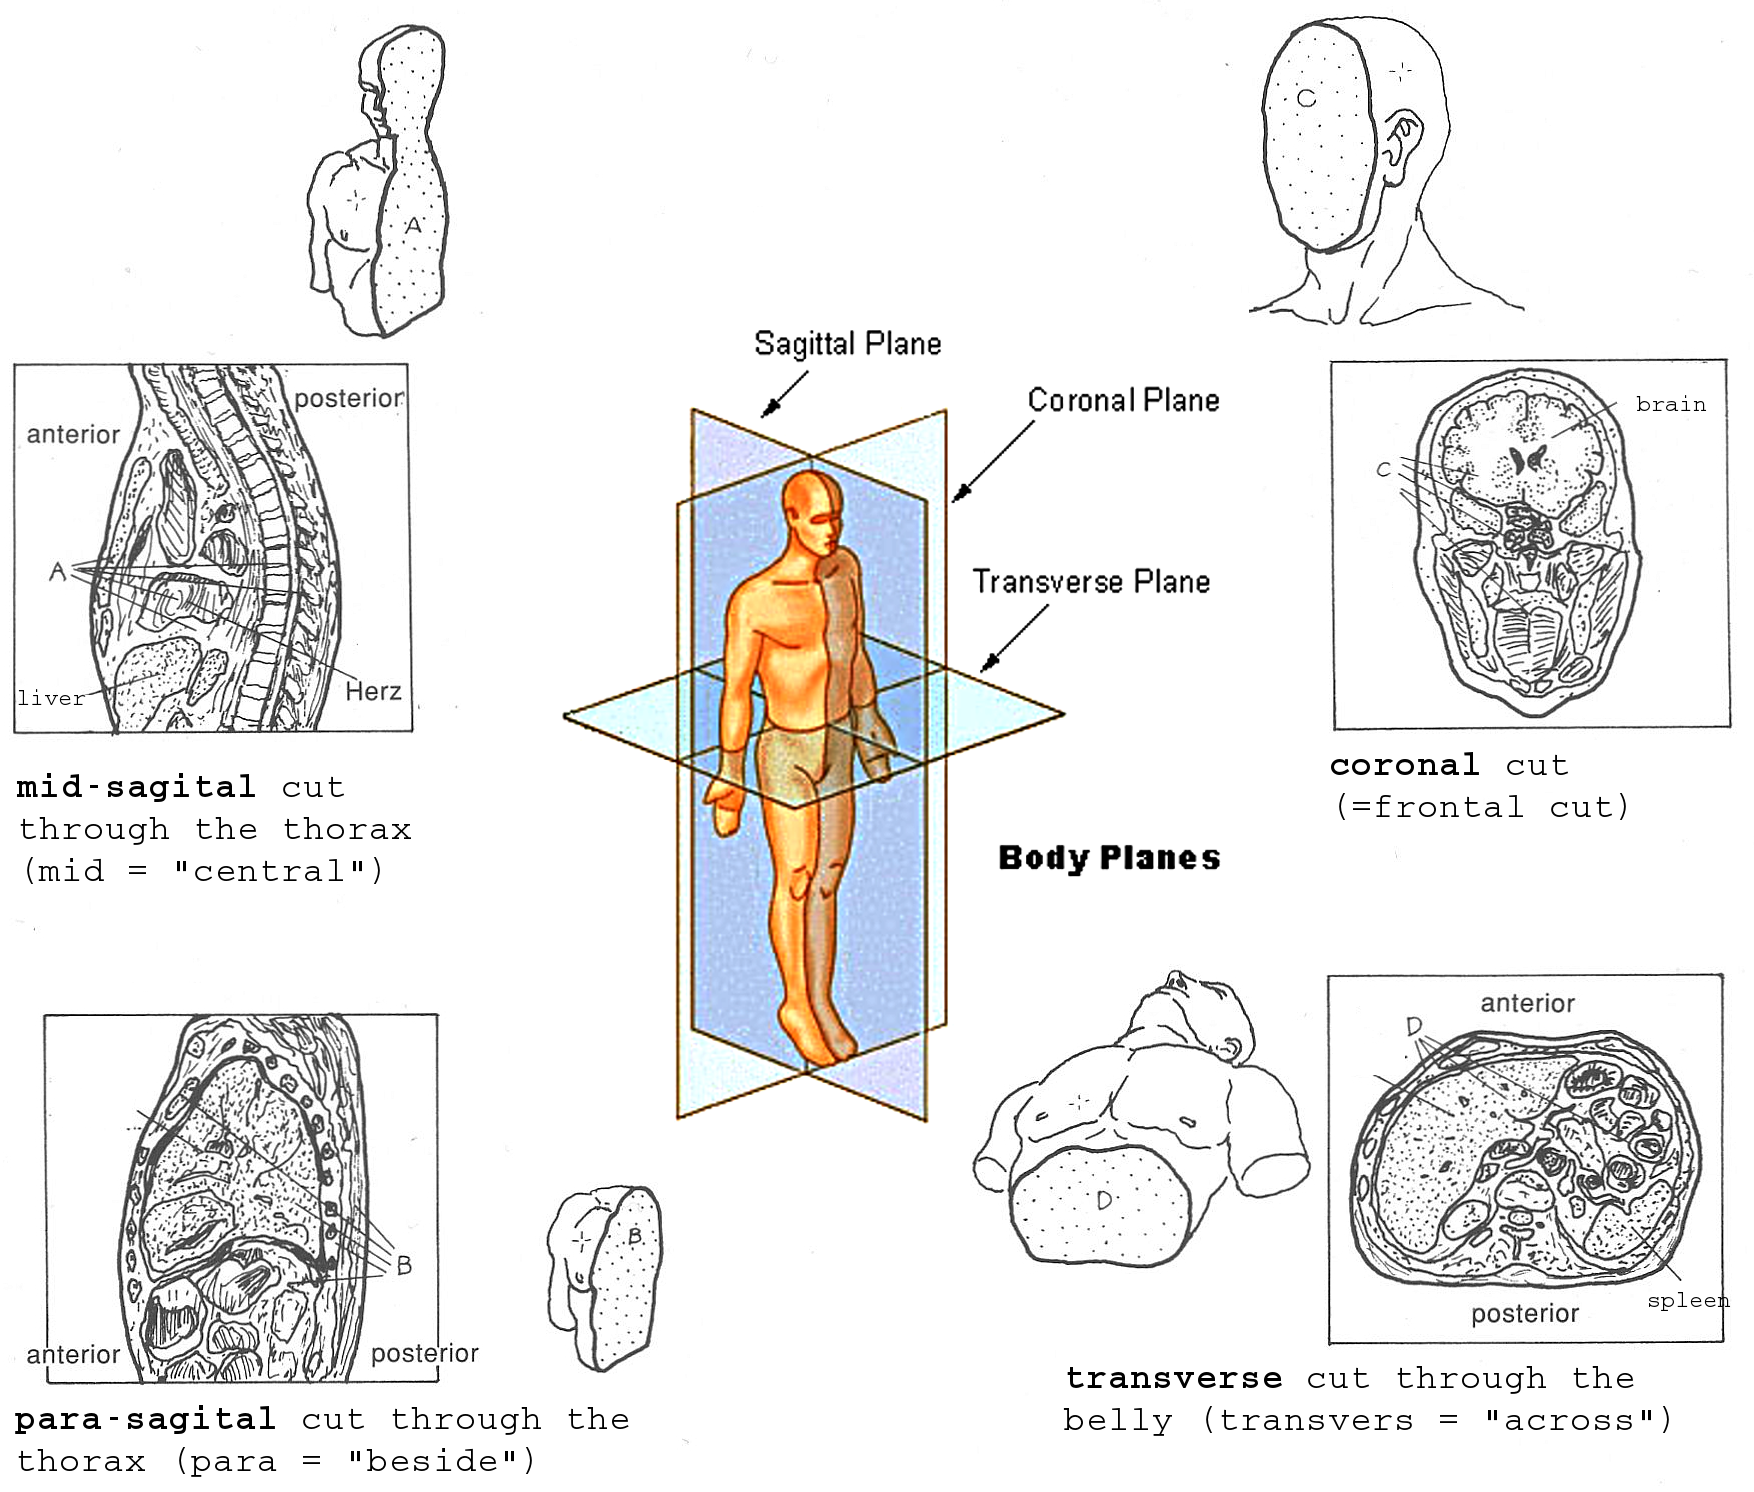
\includegraphics[width=12cm]{./Biology/hum00_anatomy/anatomical-planes-comp_v2.png}}
% 		\captionof{figure}[Anatomical planes AnatAtlas
% 		 table 1]{Anatomical planes with examples}  \label{fig:SchnittEbenen}
% 		\vspace{2pt}
% 	\end{minipage}
% 		
% 	\end{center}
% 
% 		
% 			  \begin{figure}[htbp]
% 			    \begin{minipage}{0.35\textwidth}
% 			     \centering
% 			      \includegraphics[width=1\textwidth]{./Biology/hum00_anatomy/DirectionalTerms_WikiPedia_v1.png}
% 			      \caption{Relative anatomical terms allow to describe any point of a body relative an other point, a reference.}  \label{fig:AnatomicalTerms}
% 			    \end{minipage}\hspace{0.2cm}
% 			    \begin{minipage}{0.7\textwidth}
% 			     \centering
% 			      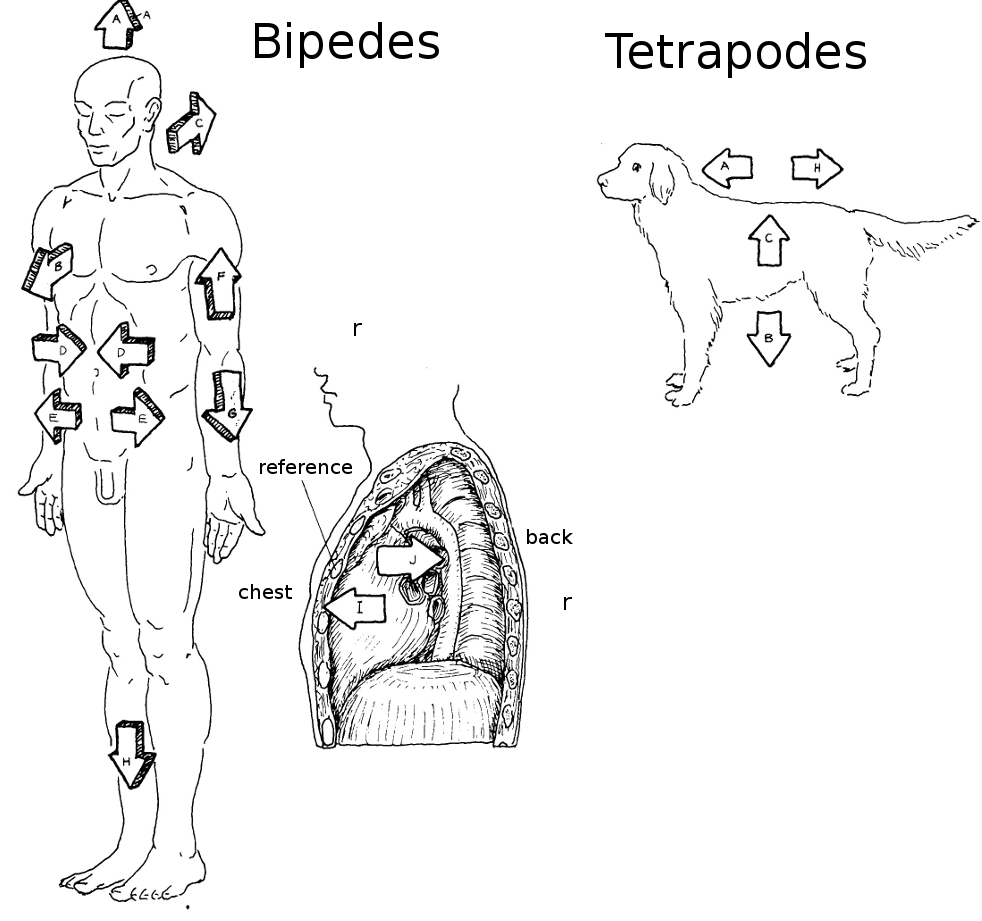
\includegraphics[width=0.9\textwidth]{/share/SB_Unterricht/Biology/hum00_anatomy/AnatomieMalatlas002_v4.png}
% 			      \caption{Asign the correct terms!}  \label{fig:AnatTermsApplication}
% 			    \end{minipage}
%  				 \end{figure}
% 		
% 
% \areaset[0cm]{11.5cm}{26.5cm}

\subsubsection*{The four body planes}\ref{sss:FourBodyPlanes}
Study of the human body requires an organized visualization of its internal parts. Dissection ("`dis"`, \textit{apart}; "`sect"`, \textit{cut}) is the term given to preparation of the body for general or specific internal inspection. Internal body structure is studied in sections cut along imaginary flat surfaces called \textbf{planes}. These planes are applied to the erect, standing body with limbs extended along the sides of the body, palms and toes forward, thumbs outward. See this \textsc{anatomical position }in the following page. Views of the internal body in life and after death can be obtained by a number of techniques that produce computer-generated representational images of human structure in series (sections) along one or more planes. These anatomic images may be produced by computerized tomography (CT) and magnetic resonance imaging (MRl). 

The \textbf{median plane} is the midline longitudinal plane dividing the head and torso into right and left halves. The presence of the sectioned midline of the vertebral column and spinal cord is characteristic of this plane. 

Planes parallel to the median plane are \textbf{sagittal}. Watch out! "'Medial"` is not a plane. The sagittal plane is a longitudinal plane dividing the body (head, torso, limbs) or its parts into left and right parts (nof halves). lt is parallel to the median plane. 

The \textbf{coronal} or frontal plane is a longitudinal plane dividing the body or its parts into front and back halves or pafts. These planes are perpendicular to the median and sagittal planes. 

The \textbf{transverse} or cross plane divides the body into upper and lower halves or parts (cross sections). This plane is perpendicular to the longitudinal planes. Transverse planes are horizontal planes of the body in the anatomical position.


% \begin{minipage}{10.5cm}\centering
% 	\includegraphics[width=1\textwidth]{/images/AnatomieMalatlas001_txt.png}
% 	\captionof{figure}[Text zu den Schnittebenen von Abb. 1 im Anatomieatlas]{Text zur Abbildung \ref{fig:SchnittEbenenRichtungen}}
% 	\label{fig:EbenenText}
% \end{minipage}
% \hspace{0.3cm}
\begin{minipage}{5cm}\centering
	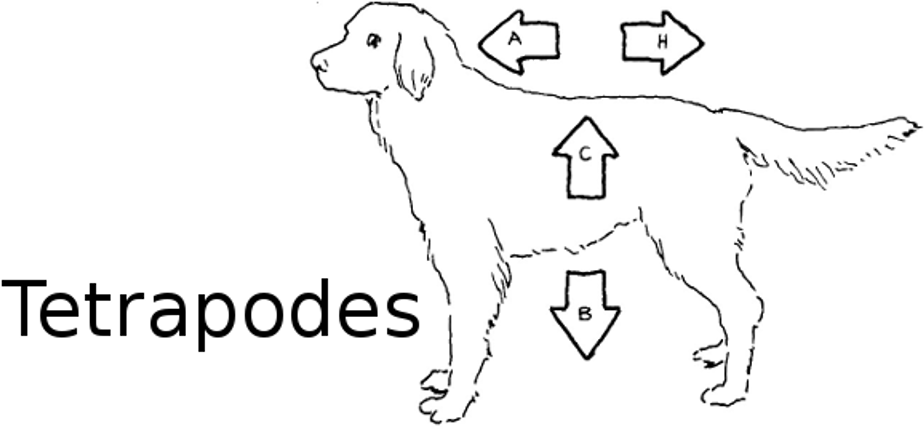
\includegraphics[width=1\textwidth]{/images/AnatomieMalatlas002_v2.png}
	\captionof{figure}[Tetrapode aus Lagebeziehungen im Anatomieatlas, S.2]{Lagebeziehungen bei einem Vierbeiner}
	\label{fig:Vierbeiner}
\end{minipage}

\areaset[1cm]{18cm}{30cm} \thispagestyle{empty}
\enlargethispage{32pt} \thispagestyle{empty}
\hspace{-0.4cm}
\begin{minipage}{6cm}
	Terms of position and direction describe the relationship of one structure on / in the body to another with reference lo the anatomical position: body standing erect, limbs extended, palms of the hands forward, thumbs directed outwardly. 
	
	\textbf{Cranial} and superior refer to a structure being closer to the top of the head than another structure in the head, neck, or torso (excluding limbs). 
	
	\textbf{Anterior or ventral} refers to a structure being more in front than another structure in the body. 
	
% 	\textbf{Ventral} refers to the abdominal side; in bipeds, it is synonymous with anterior. 
	
% 	\textbf{Rostral} refers to a beak-like structure in the front of the head or brain that projects forward. 
	
	\textbf{Posterior and dorsal} refer to a structure being more in back than another structure in the body. Dorsal is synonymous with posterior (the preferred term) except in quadrupeds. 
	
	\textbf{Medial} refers to a structure that is closer to the median plane than another structure in the body. 
	
	\textbf{Lateral} refers to a structure that is farther away from the median plane than another structure in the body.
	
	 Employed only with reference to the limbs, \textbf{proximal} refers to a structure being closer to the median plane or root of the limb than another structure in the limb. Employed only with reference to the limbs, \textbf{distal} refers to a structure being farther away from the median plane or the root of ihe limb than another structure in the limb. 
	 
	 \textbf{Caudal} and inferior refer to a structure being closer to the feet or the lower part of the body than another structure in the body. These terms are not used with respect to the limbs. In quadrupeds, caudal means closer to the tail. 
	 
% 	 The term superficial is synonymous with exfernal, the term deep with internal. Related to the reference point on the chest wall, a structure closer to the surface of the body is superficial; a structure further away from the surface is deep. Ipsilateral means "on the same side" (in this case, as the reference point); contralateral means "on the opposite side" (of the reference point). The quadruped presents four points of direction: head end (cranial), tail end (caudal), belly side (ventral), and back side (dorsal).
\end{minipage}
\hspace{0.3cm}
\begin{minipage}{9cm}
	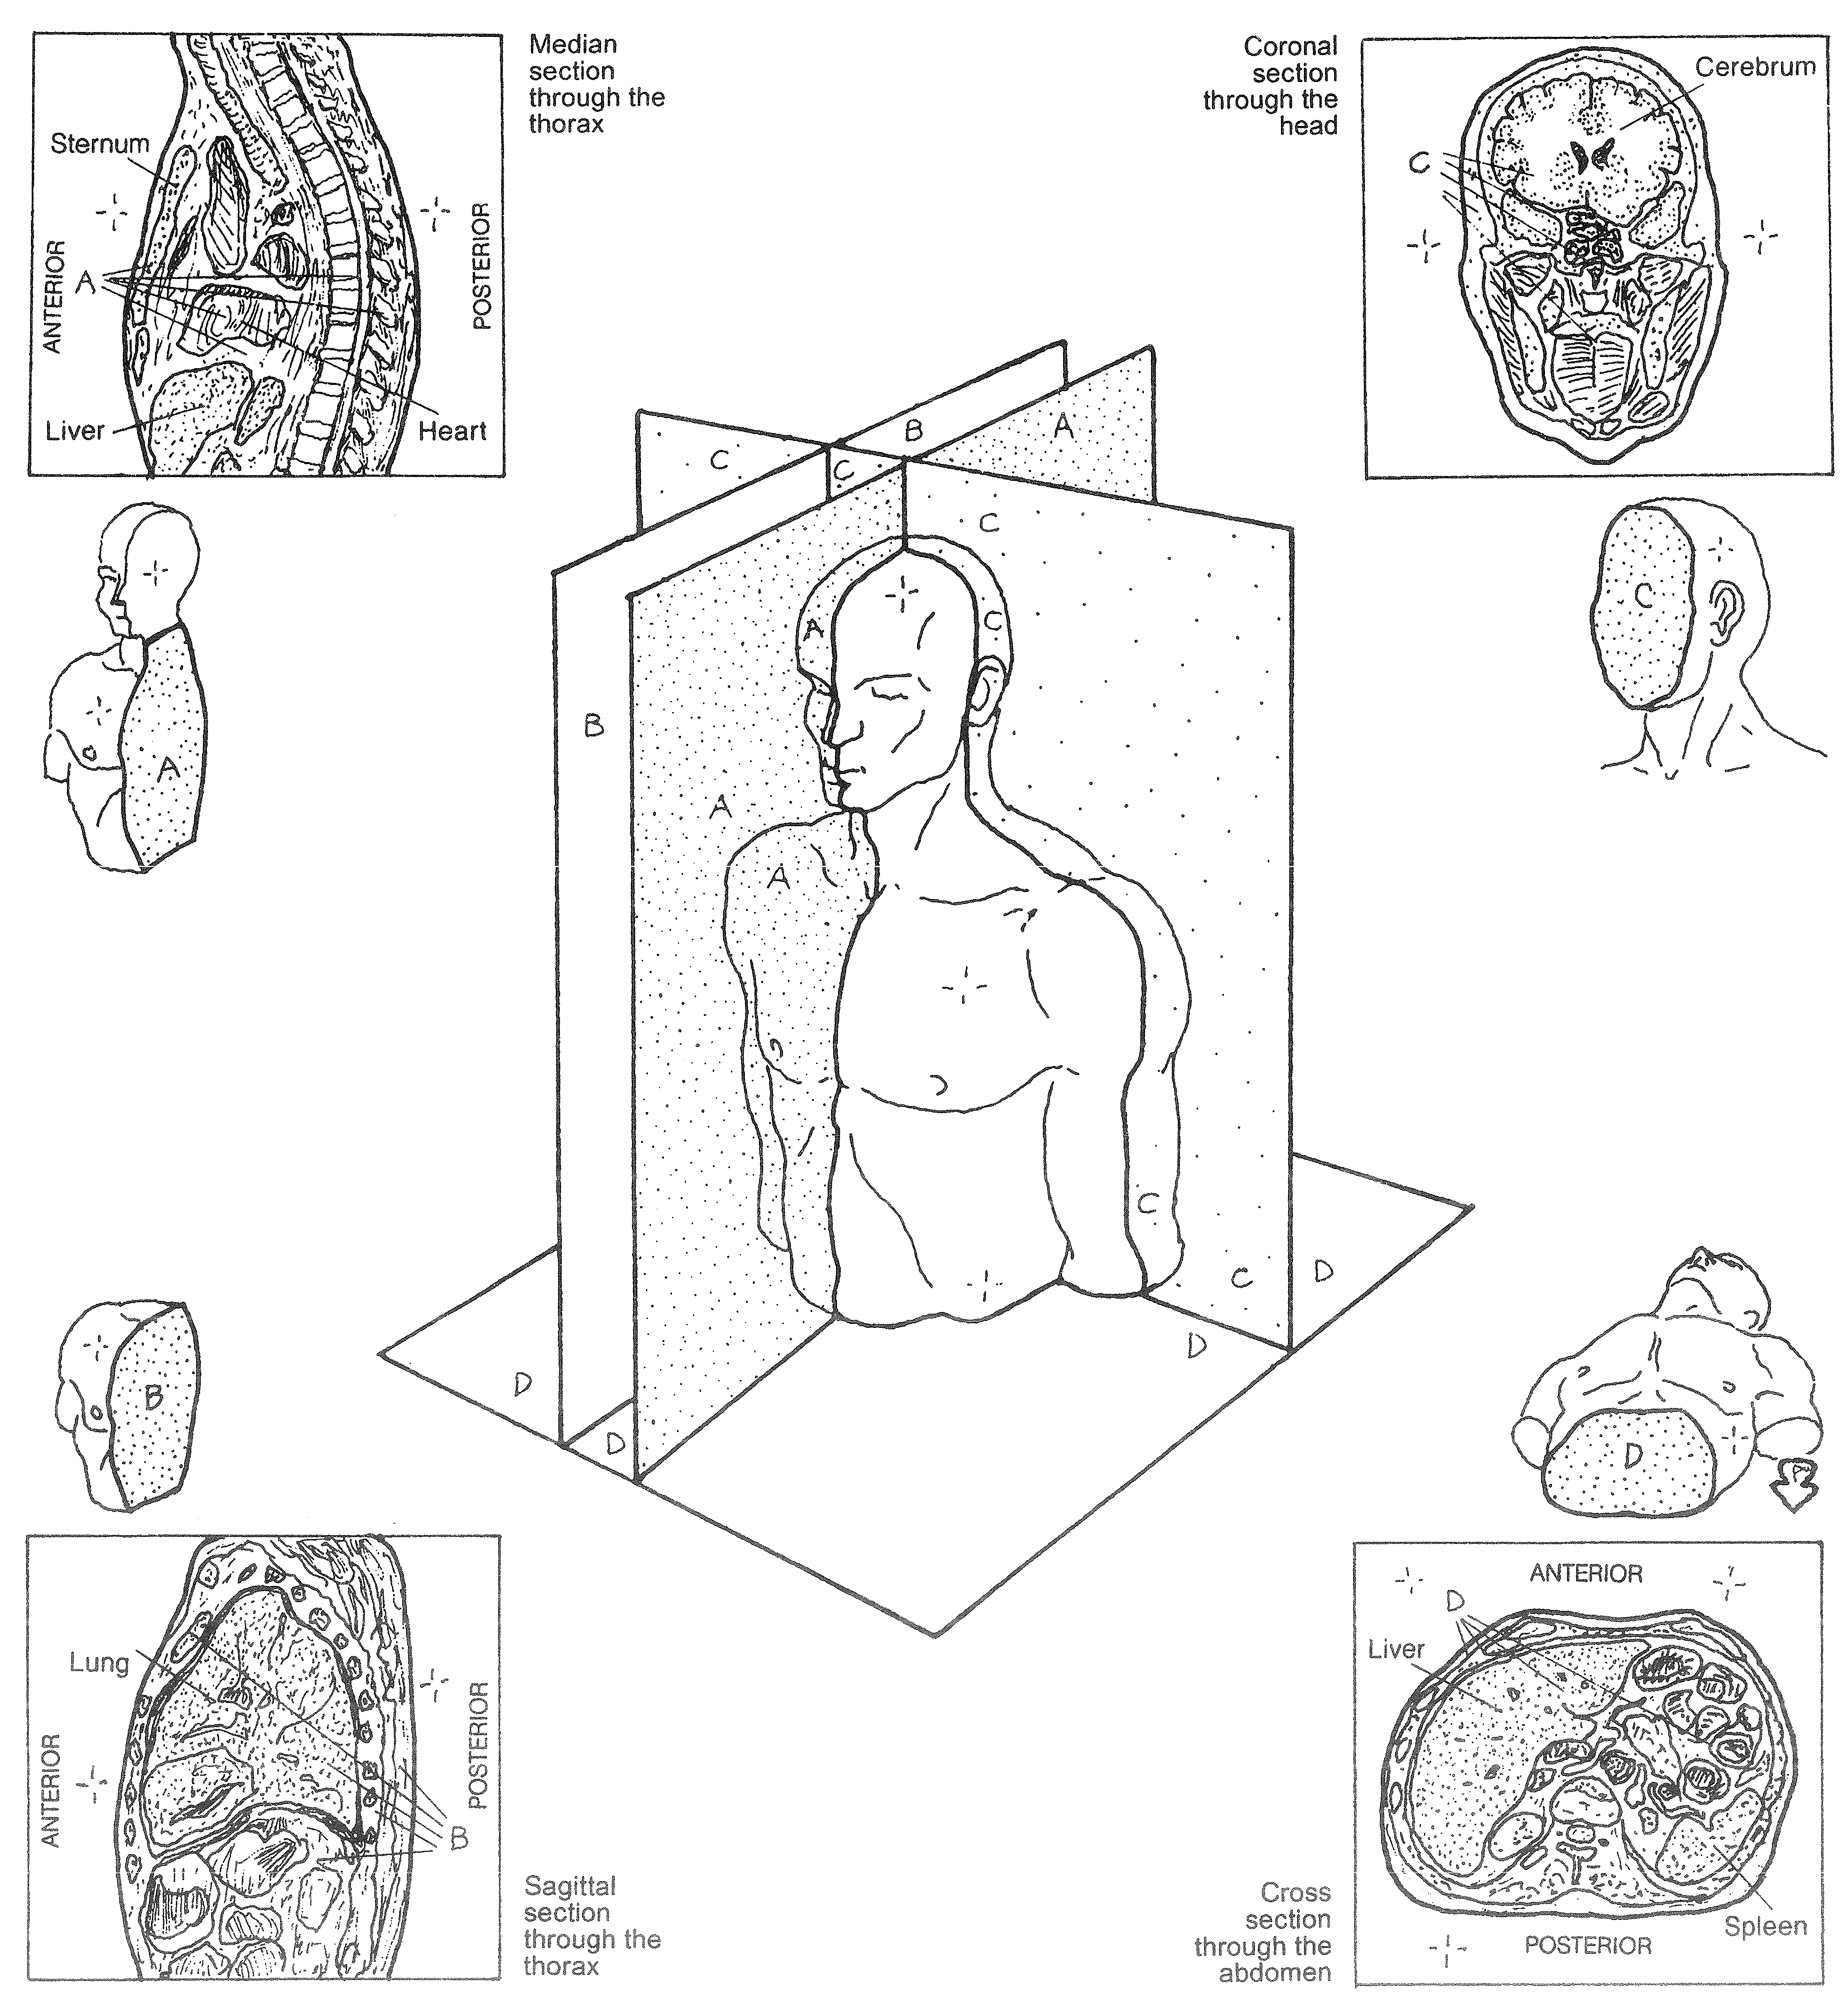
\includegraphics[width=1\textwidth]{/share/00_SCHULE_DATA-add/bilder_saz/Humanbio_Bilder/Anatomie_MalAtlas_en/2nd-edition/AnatCol-4ed_001_v1.png}
	\captionof{figure}[aus malatlas-en fig. 001]{The four body planes}
	\label{fig:BodyPlanesAnatAtl}
 		\centering
		{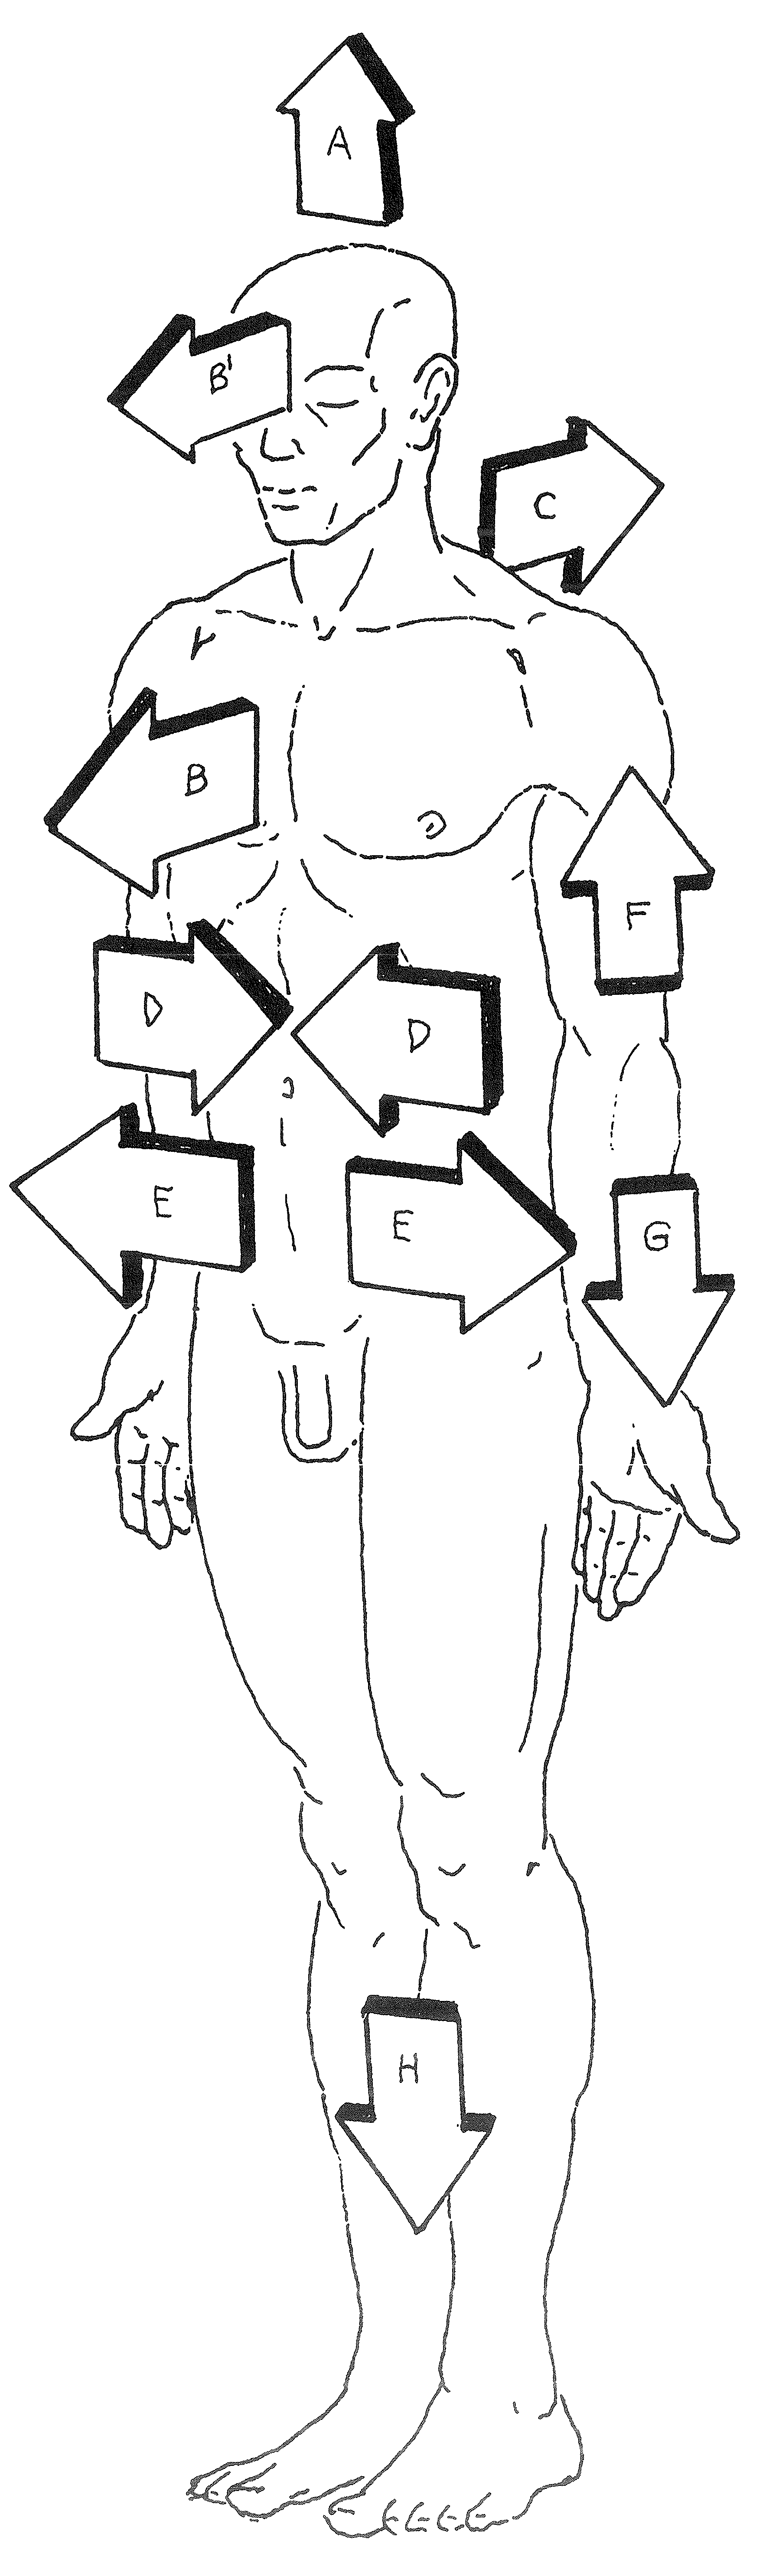
\includegraphics[width=0.5\textwidth]{/share/00_SCHULE_DATA-add/bilder_saz/Humanbio_Bilder/Anatomie_MalAtlas_en/2nd-edition/AnatCol-4ed_002_v1.png}}
		\captionof{figure}[terms of direction anat atlas 4th p002]{Anatomical terms of direction}  \label{fig:AnatDirections}
		\vspace{2pt}
	\end{minipage}
  


%********************************************************
 \areaset[0cm]{18cm}{26cm}
\begin{landscape} \thispagestyle{plain}
	\hspace{-2cm}
	\begin{minipage}{26cm}
	\begin{multicols}{3}[\subsection{The eleven organ systems}\label{ssc:AnatOrgansysteme}]
		The multitude of tissues and organs can be organised in ten organ systems. \textit{Solution texts in the table taken from Russel, Dynamic Science, chapter 38; "'interactions"` copied mainly from \url{https://www.wsfcs.k12.nc.us/cms/lib/NC01001395/Centricity/Domain/8472/Body\%20Systems\%20Interactions\%20chart.pdf}  }%
		\columnbreak

		Use the learning cards alongside: \href{/share/SB_Unterricht/Biology/hum00_anatomy/11-Organsystems-cards_HS18.sla}{11-Organsystems-cards\_HS18 as pdf written in scribus}
	\end{multicols}	
	\end{minipage}
	 
%% Erste von zwei Tabellen  %%%%%%%%%%%%%%%%%%%%%%%%%	

	\Ersatz{	 \hspace{-2cm}
	\begin{minipage}{26.5cm}
% 	 \begin{table}
		 \captionof{table}{The eleven organ systems}
  		  \setlength{\extrarowheight}{0pt}
  \begin{tabularx}{26cm}[]{m{1.6cm} m{2.4cm} m{4cm} m{7cm} m{8.5cm}}
	\toprule
	 pict & system & parts & task \& functions & interactions \\\midrule
	
	 \includegraphics[height=2.5cm]{/images/figures/Russel-38_10_01.png}
	& Nervous System &  Brain, spinal cord,  peripheral nerves,  sensory organs &
	Principal regulatory  system; monitors  changes in internal  and external  environments and  formulates  compensatory  responses; responsible for instinctive and learned behaviors; coordinates body  activities & Controls all other systems; Hypothalamus maintains homeostasis by working with all systems.   \\  \midrule

	\includegraphics[height=2.4cm]{/images/figures/Russel-38_10_02.png}
	& Endocrine System (ES) &  Pituitary gland, hypothalamus, thyroid gland,  adrenal gland, pancreas,  and other hormone-secreting glands& Regulates and  coordinates body  activities through  secretion of  hormones; long lasting but slow acting & 1. circulatory: transports hormones to target organs. ~ 2. nervous:  maintain homeostasis, hormone release. ~ 3. reproductive: ES controlled by hormones. ~ 4. skeletal: ES controls growth of bones.  \\  \midrule

	\includegraphics[height=2.4cm]{/images/figures/Russel-38_10_03.png}
	& Muscular System  & Skeletal, cardiac, and smooth muscle & Moves body parts;  helps run bodily  functions; generates  heat; moves intestinal lumen contents & 1. skeletal: allow movement; ~ 2. digestive: allow organs to contract to push food through; ~ 3. respiratory: diaphragm (muscle) controls breathing; ~ 4. circulatory: controls pumping of blood (heart muscle); ~ 5. nervous: controls all muscle contractions   \\  \midrule

	\includegraphics[height=2.4cm]{/images/figures/Russel-38_10_04.png}
	& Skeletal System (SK)  & Bones, tendons,  ligaments, cartilage &Supports and  protects body parts;  provides leverage for  body movements;  stores minerals & 1. muscular: allow movement 2. circulatory: SK produces red blood cells 3. immune: SK produces white blood cells 4. circulatory and respiratory: SK protects it’s organs and opens the chest's volume  \\  \midrule

	\includegraphics[height=2.4cm]{/images/figures/Russel-38_10_05.png}
	& Integumentary System  & Skin, sweat glands, hair, nails & Covers external body surfaces and  protects against  injury and infection;  helps regulate water  content and body  temperature & 1. excretory: removes cellular waste; 2. nervous: controls body temperature (sweating, goose bumps) 3. immune: prevents pathogens from entering ("'first line of defense"`)  \\  \midrule
	\bottomrule
	\end{tabularx}%
	  \label{tab:ZehnOrgansysteme}%
% 		 \end{table}
	\end{minipage}
	}{
	\hspace{-2.2cm} \begin{minipage}{26.5cm}
	 \captionof{table}{The eleven organ systems}
  		  \setlength{\extrarowheight}{0pt}
  \begin{tabularx}{26cm}[]{m{1.6cm} m{2.4cm} m{4cm} m{7cm} m{8.5cm}}
	\toprule
	pict & system & parts & task \& functions & interactions \\\midrule

			\includegraphics[height=2.4cm]{/images/figures/Russel-38_10_01.png}
			   & & & & \\  \midrule
			\includegraphics[height=2.4cm]{/images/figures/Russel-38_10_02.png}
			 & & & & \\  \midrule
			
			\includegraphics[height=2.4cm]{/images/figures/Russel-38_10_03.png}
			  & & & & \\  \midrule

			\includegraphics[height=2.4cm]{/images/figures/Russel-38_10_04.png}
			 & & & & \\  \midrule

			\includegraphics[height=2.4cm]{/images/figures/Russel-38_10_05.png}
			  & & & & \\ 
	\bottomrule
	\end{tabularx}%
	  \label{tab:ZehnOrgansysteme}%
% 		 \end{table}	
	\end{minipage}
	}
	 \end{landscape}
%%% Zweite von zwei Tabellen %%%%%%%%%%%%%%%%%%%%%%%%%%	 
		 
 \areaset[0cm]{19.4cm}{26cm} \begin{landscape}	\thispagestyle{plain}\enlargethispage{1cm}
\Ersatz{ \hspace{-2.2cm}
	\begin{minipage}{26.5cm}
	 \captionof{table}{The eleven organ systems (cont.)}
  	 \setlength{\extrarowheight}{0pt}
     \begin{tabularx}{26cm}[]{m{1.5cm} m{2.2cm} m{4.3cm} m{7cm} m{9cm}}
		\toprule 
		 pict & system & parts & task \& functions & interactions \\\midrule

	\includegraphics[height=2.4cm]{/images/figures/Russel-38_10_06.png}
	& Cardiovascular System  & Heart, blood  vessels, blood & Distributes water,  nutrients, oxygen,  hormones, and other substances  throughout body  and carries away  carbon dioxide and  other metabolic  wastes; helps  stabilize internal  temperature and pH-value & 1. Respiratory: deliver \ce{O2} from lungs to cells and drop off \ce{CO2} from cells to lungs. 2. Digestive: absorb digested nutrients and deliver to cells. 3. Excretory: kidneys filter waste out of blood. 4. Lymphatic: takes up excess plasm. 5. Immune: transports white blood cells to fight disease. 6. Nervous: brain controls heartbeat. 7. endocrine: transport of hormones   \\  \midrule

		\includegraphics[height=2.4cm]{/images/figures/Russel-38_10_07.png}
		& Lymphatic (\textit{immune}) System  & The lymph fluid, network of lymph vessels and nodes, white blood cells; specialised organs: spleen, thymus, bone marrow.  & Produces and transports the fluid lymph which contains white blood cells; defends against  disease-causing  microorganisms  and viruses  (pathogens); Removes excess lymph from these places between body tissues and returns it to the blood. & 1. circulatory: transports white blood cells to fight invaders 2. lymphatic: has lots of white blood cells to fight invaders and the spleen filters bacteria and viruses out of blood 3. skeletal: whit blood cells made in bone marrow 4. integumentary: prevents invaders from getting into the body. \\  \midrule
		
		\includegraphics[height=2.4cm]{/images/figures/Russel-38_10_08.png}
		& Respiratory System  & Lungs, diaphragm, trachea, and other airways & Exchanges gases  with the  environment, including uptake of oxygen and release  of carbon dioxide  & 1. Circulatory System: takes in \ce{O2} for delivery to cells and removes \ce{CO2} brought from cells. ~ 2. Excretory System: removes waste via the lungs. ~3. Nervous System: controls breathing.~ 4. Muscular System: controls breathing through the diaphragm (muscle). \\  \midrule
		
		\includegraphics[height=2.4cm]{/images/figures/Russel-38_10_09.png}
		& Digestive System  & Oral cavity, pharynx,  esophagus, stomach, intestines, liver,  pancreas, rectum, anus & Converts ingested matter into  molecules and ions that can be  absorbed into body;  eliminates  undigested matter; helps regulate water content & 1. circulatory: absorb \& deliver the digested nutrients to the cells 2. muscular: control the contractions of many of the digestive organs to pass food along 3. nervous: hypothalamus maintains homeostasis by triggering appetite (stomach growling). \\  \midrule
		
		\includegraphics[height=2.4cm]{/images/figures/Russel-38_10_10.png}
		& Urinary System  &  Kidneys, bladder,  ureter, urethra & Removes and eliminates excess water, ions, and  metabolic wastes from body; helps regulate internal osmotic balance  and pH; helps regulate blood pressure & 1. circulatory: filters waste out of blood; 2. lungs: removes excretory waste; 3. integumentary: removes excretory waste \\  \midrule
		
		\includegraphics[height=2.4cm]{/images/figures/Russel-38_10_11.png}
		& Reproductive System  &Female: ovaries, oviducts, uterus, vagina, mammary  glands Male: testes, sperm ducts,  accessory glands, penis& Maintains the sexual characteristics and passes on genes to the next generation & 1. endocrine: controls production of sex cells.  2. muscular: uterus contracts to give birth - controlled by hormones (endocrine) \\
		\bottomrule
	\end{tabularx}%
	  \label{tab:ZehnOrgansystemeCont}%
		 \end{minipage}
		  }{
	\hspace{-2.2cm} \begin{minipage}{26.5cm}
	 \captionof{table}{The eleven organ systems (cont.)}
  	 \setlength{\extrarowheight}{9pt}
     \begin{tabularx}{26cm}[]{m{1.6cm} m{2.4cm} m{4cm} m{7cm} m{8.5cm}}
		\toprule 
		 Bild & Organsystem & Funktion &  weitere Aufgaben & Besonderes  \\\midrule
		\includegraphics[height=2.5cm]{/images/figures/Russel-38_10_06.png}
		  & & & & \\  \midrule
		
		\includegraphics[height=2.5cm]{/images/figures/Russel-38_10_07.png}
		  & & & & \\  \midrule
		
		\includegraphics[height=2.5cm]{/images/figures/Russel-38_10_08.png}
		  & & & & \\  \midrule
		
		\includegraphics[height=2.5cm]{/images/figures/Russel-38_10_09.png}
		 & & & & \\  \midrule
		
		\includegraphics[height=2.5cm]{/images/figures/Russel-38_10_10.png}
		 & & & & \\ \midrule

		\includegraphics[height=2.5cm]{/images/figures/Russel-38_10_11.png}
		 & & & & \\  \midrule
		\bottomrule
	\end{tabularx}%
	  \label{tab:ZehnOrgansystemeCont}%
		 \end{minipage}

		 }%		 
\end{landscape}

 \areaset[0cm]{18cm}{28cm} \begin{landscape} \thispagestyle{plain}
	\begin{enumerate}[resume, leftmargin=*]   %  <ctrl-alt-i>  für "item"
		\item Übertragen Sie fünf der zehn Organsyteme in die nachfolgenden Figuren: Herz-Kreislauf-System; Endokrines System; Verdauungssystem; Atemsystem; Harnsystem
	\end{enumerate}

% \enlargethispage{4ex}

\vspace{4ex}
% \hspace{-1cm}
\begin{minipage}{8cm} \centering
\begin{overpic}[angle=0,scale=1.2,grid,tics=12.5]%
{/share/00_SCHULE_DATA-add/bilder_saz/Humanbio_Bilder/Humanbio_Smith/smith10-2_sw.jpg}
\end{overpic}
%\captionof{figure}[Anatomie Figuren aus Smith mit 8x4 Raster ]{Mit Hilfe eines 8 x 4 Rasters  kann man sich die Proportionen der menschlichen Gestalt sehr gut merken.}	\label{fig:RasterFiguren}
\end{minipage}
\hspace{1cm}
\begin{minipage}{8cm} \centering
\begin{overpic}[angle=0,scale=1.2,grid,tics=12.5]%
{/share/00_SCHULE_DATA-add/bilder_saz/Humanbio_Bilder/Humanbio_Smith/smith015-2_sw_v2.jpg}
\end{overpic}
\end{minipage}
\hspace{0.6cm}
\begin{minipage}{8cm} \centering
\begin{overpic}[angle=0,scale=1.2,grid,tics=12.5]%
{/share/00_SCHULE_DATA-add/bilder_saz/Humanbio_Bilder/Humanbio_Smith/smith015-XX_sw.jpg}
\end{overpic}
\end{minipage}
\end{landscape}

 \areaset[0cm]{18cm}{28cm} \begin{landscape} \thispagestyle{plain}
\vspace{3ex}
\hspace{-1cm}
\begin{minipage}{8cm} \centering
\begin{overpic}[angle=0,scale=1.2,grid,tics=12.5]%
{/share/00_SCHULE_DATA-add/bilder_saz/Humanbio_Bilder/Humanbio_Smith/smith015-2_sw_v2.jpg}
\end{overpic}
\end{minipage}
\hspace{0.6cm}
\begin{minipage}{8cm} \centering
\begin{overpic}[angle=0,scale=1.2,grid,tics=12.5]%
{/share/00_SCHULE_DATA-add/bilder_saz/Humanbio_Bilder/Humanbio_Smith/smith015-XX_sw.jpg}
\end{overpic}
\end{minipage}
\hspace{1cm}
\begin{minipage}{8cm} \centering
\begin{overpic}[angle=0,scale=1.2,grid,tics=12.5]%
{/share/00_SCHULE_DATA-add/bilder_saz/Humanbio_Bilder/Humanbio_Smith/smith015-2_sw_v2.jpg}
\end{overpic}
\end{minipage}
	
	\vspace{1cm}
	\begin{enumerate}[resume, leftmargin=*]   %  <ctrl-alt-i>  für "item"
		\item Vergrössern Sie eine der in Abb. \ref{fig:RasterFiguren} abgebildeten leeren Figuren auf ein A3-Papier mit derselben Rastereinteilung. Zeichnen sie in ihre vergrösserte Figur die folgenden Organe ein: \textbf{Lungen, Thymus, Herz, Leber, Zwerchfell, Hirn, Milz, Oberschenkelknochen mit Mark, Blase und Nieren} ein. Achten Sie auf die Körperproportionen und die korrekte Lage der Organe. Diese Darstellung geben Sie bis zum vereinbarten Datum ab - sie wird bewertet.
	\end{enumerate}
	
\end{landscape}
		
% %%%  ein A3-Papier-Raster nötig!! %%%%		
% 		\enlargethispage{4ex}	
% 			\vspace{4pt}
% 		
% 			 \begin{center}
% 				\begin{minipage}[htbp]{1\columnwidth}
% 			 \centering
% 				\begin{tikzpicture}[scale=2.9]
% 					\draw (0,0) grid (4,8);
% 				\end{tikzpicture}
% 					\captionof{figure}[8x4 Raster tzkip-pict]{Raster für eine anatomische Figur - vgl. Abb. \ref{fig:RasterFiguren}}  \label{fig:AnatRaster}
% 				\end{minipage}
% 					\marginline{\todol{extra Kopie für SuS!}}
% 			  %\hfill 
% 			 \end{center}





